\documentclass{article}

\usepackage[utf8]{inputenc}
\usepackage{graphicx}
\usepackage[margin=0.6in]{geometry}

\usepackage[style=numeric, sorting=none]{biblatex}
\addbibresource{bibliography.bib}

\usepackage{hyperref}
\usepackage[justification=centering]{caption}
\usepackage{subcaption}
\usepackage{amsmath}
\usepackage[subtle]{savetrees}

\hypersetup{
    colorlinks=true,
    linkcolor=black,
    urlcolor=blue,
    citecolor=black
}


\title{Does Crime Pay? Co-Evolution of Insider Trading and its Regulation}
\author{Jagdev Bal, Ellie Fadipe, Jade Jones, Alex Room}
\date{}

\begin{document}

\maketitle
\textbf{Abstract}:
We model the co-evolution of insider trading and trade regulation in a financial market with a \emph{paired Moran process}, a variant on the graph-based Moran process for asymmetric games. We find that the most effective regulation strategies take care not to over-investigate, but punish repeat offenders; the most effective trading strategies either avoid insider trading altogether or 'strategically exploit' the market.

\section{Introduction}
Insider trading is the practice of buying or selling a company’s securities\footnote{i.e. assets which can be traded on a financial market} while in possession of information that is not yet public (e.g. learning about a company's merger via dinner with the CEO). This practice may be illegal but is not uncommon in today's markets; insider traders enjoy better returns with less risk \parencite{bainbridge1998insider}. This project sets out to investigate the relationship between strategies for both insider trading and its regulation. We test the effectiveness of a number of different strategies between insider traders and regulators under a co-evolutionary dynamic to see if there are superior strategies to both detect and avoid detection. 

Similar studies include \textcite{smales2017game}, who model a similar scenario using Monte Carlo simulation. We instead use evolutionary dynamics to model these interactions.

\section{Methods, Strategy \& Evolution}
Our stage game has two players, a trader $\mathcal{T}$ and a trading regulator $\mathcal{R}$ who are the row and column players respectively; the trader's actions as a 'regular' vs an 'insider' trade; the regulator's actions as 'no investigation' vs 'investigation'; and financial payoff matrices for both players as follows:
\begin{equation*}
\begin{split}
    \mathcal{T}: 
    \begin{pmatrix}
    1 & 1 \\
    6 & -10
    \end{pmatrix}
\end{split}
\quad\quad
\begin{split}
    \mathcal{R}: 
    \begin{pmatrix}
    1 & -1 \\
    -3 & 5
    \end{pmatrix}
\end{split}
\end{equation*}

i.e. a 'regular' trade has a small financial gain, but is immune to investigation -- an insider trade, on the other hand, is much more lucrative but sustains heavy fines if caught. The regulator is punished on 'false positive' investigations and on failing to catch insider traders\footnote{Statistical methods such as those in \textcite{bris2005insider} can recognise that insider trading has occurred through passive stock market analysis, but not who is doing it.}, but are rewarded for catching fraud. 

We note that in the scenario we are modelling, the two players do not have equal information. The trader always knows when they have been investigated, but the regulator can only be certain the trader has done insider trading if they have caught them doing it! Compare this to the Prisoner's Dilemma, where both players have full information.
\newline\\
\noindent\textbf{Strategy \& Evolution}

We then create strategies for our game using the Axelrod library \parencite{axelrodproject}. We have written code\footnote{available at \href{https://github.com/alexhroom/gametheory}{https://github.com/alexhroom/gametheory}} to implement asymmetric games into the library, and then used tournaments in those asymmetric games (iteratively playing each trader against each regulator) to simulate a 'paired Moran process', which simplifies the graph-based Moran process of \textcite{shakarian2013novel}. We take two populations -- $P_1$ of row players, and $P_2$ of column players -- and calculate the fitness of each member of each population against the \emph{other} population. With the Hawk-Dove game as an example, if $P_1 = \{\text{2 hawk, 1 dove}\}$ and $P_2 = \{\text{1 hawk, 2 dove}\}$, the fitness of the dove in $P_1$ is calculated based on its utilities against the 1 hawk and 2 doves in $P_2$. Birth and death is then calculated for each population from these fitnesses in the same way as the regular Moran process. We do this independently for each population (1 birth and 1 death in $P_1$, \emph{and} 1 birth and 1 death in $P_2$)

As opposed to the usual Moran process, this allows us to simulate situations where it may not be suitable for every player to interact with every other player; traders and regulators do not interact among themselves in the situation we are modelling, and asymmetric information means they do not necessarily share strategy spaces. This provides insight into how trading behaviour co-evolves with regulation behaviour over time, as separate yet dependent populations.

The final scores of each matchup in the tournament take an average of 500 matches of 500 iterations each; the iterations model consecutive trading days. We used 6 trading strategies, and 5 regulation strategies. We ran 220 repeats of the process.

\section{Results}
\begin{figure}[!h]
  \begin{subfigure}[c]{0.5\textwidth}
    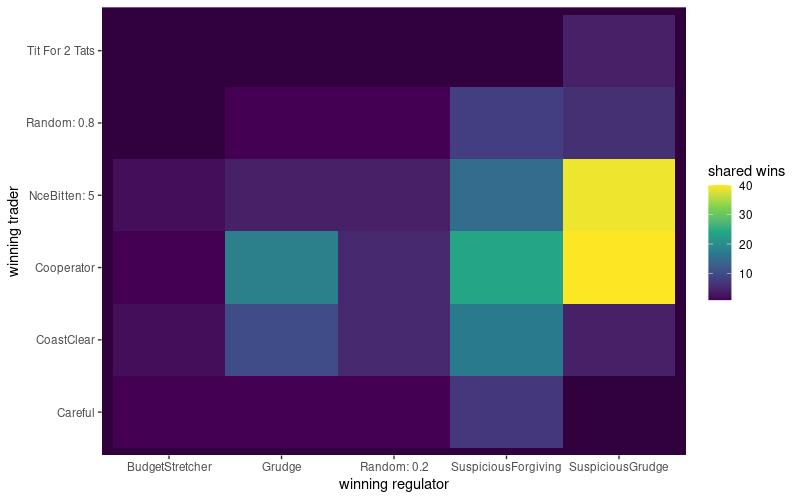
\includegraphics[width=\textwidth]{heatmap.png}
    \caption{A heatmap of co-winning trader-regulator pairs}
    \label{fig:f1}
  \end{subfigure}
  \hfill
  \begin{subfigure}[c]{0.5\textwidth}
    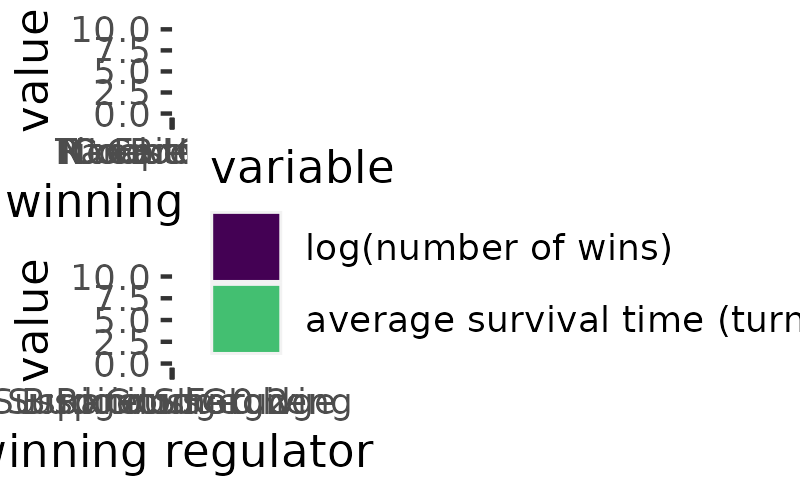
\includegraphics[width=\textwidth]{barplot.png}
    \caption{The number of wins (log base 10) and average survival time (in turns) of each trader/regulator}
    \label{fig:f2}
  \end{subfigure}
\end{figure}

We find that the most successful trading strategy is the \texttt{Cooperator} strategy, who never inside trades, followed by the \texttt{NceBitten:5} strategy, who inside trades constantly until caught 5 times, then cooperates forever; note in figure (\ref{fig:f1}) that this strategy performs almost as well as the leading strategy against the most successful regulator, but distinctly worse against the rest. The most successful regulation strategies were the \texttt{Suspicious} strategies, who track a 'suspicion' probability which increases and decreases based on the traders' patterns and investigates proportionally to suspicion. The more successful of the two was the \texttt{Grudge} variant, which raises suspicion to 100\% after catching a trader, whereas \texttt{Forgiving} lowers it to 20\%.; surprisingly, while \texttt{SuspiciousGrudge} did the best, the similar \texttt{Grudge} performed less well. This strategy investigates randomly but investigates constantly after catching the trader once.

A point of interest is that the best three trading strategies are one which never inside trades, and two which inside trade as often as possible up to a condition -- the third best was \texttt{CoastClear}, which inside trades \emph{every turn} unless they were investigated on the previous turn -- yet \texttt{Careful}, which trades inversely proportional to the \texttt{Suspicious} regulator's investigation probability, did worse than random trading, despite being written specifically as a counter to the \texttt{Suspicious} strategies.

\section{Conclusion}
We find that insider trading and its regulation co-evolves such that the best regulation strategies take care not to over-investigate, but punish repeat offenders; in tow, the best traders avoid building up a 'reputation' for insider trading. Indeed, more complex models such as those in \textcite{kyle1985continuous} suggest the power of 'strategic exploitation' as shown in our successful \texttt{CoastClear} and \texttt{NceBitten:5} strategies, although the most powerful strategy was to not inside trade at all -- this is unsurprising as if no insider traders exist, all regulation just wastes money -- but it does show that insider traders do not necessarily have an advantage over regular traders!

Returning to the previously mentioned paper by \textcite{smales2017game}, we see similarly to their investigation that regulation is, in general, not hugely effective; if it were, figure (\ref{fig:f2}) would have the number of wins inversely proportional to how often they inside trade. Reaching a similar conclusion suggests that the paired Moran process is a fruitful method of game theoretic investigation of separate, dependent populations; an interesting further investigation would be to follow this study's lead by varying the utility of punishment for insider trading and analysing its effect on dominant trading strategies.
\begingroup
\setlength\bibitemsep{0pt}
\printbibliography
\endgroup

\end{document}
